\chapter{Prototype} % Main chapter title
Vi må vell kanskje rename denne seksjonen ,til graphs eller noe. Ettersom det er jo egentlig ikke prototypen som er i fokus
\label{chapter5} % For referencing the chapter elsewhere, use \ref{Chapter1} 

\section{Initial Graphs}
\label{sec:initialGraphs}

%We must settle on a name for these types of graphs
\subsection{Fractional charts}
These types of charts shows the sum of time spent sedentary, standing, and walking. Summing over the three classifications makes it easy to get an overview of the day as a whole. Though the summation gives a great overview, details are lost and it is not possible to pinpoint when each activity occurred during the day. (Name of chart)* can be useful for quickly identifying days with a low amount of activity, before spending time looking at more detailed visualisations. It might also serve as an alert for subjects with a low activity level.

\subsubsection{Pie chart}
The pie chart is a standard way of showing fraction of time spent on each behavioural pattern. The overall design of the pie chart is very standard. We decided to create a separate legend instead of writing a descriptive text on different pie slices. The legend is a simple box which connects a behavioural pattern to each colour. The exact percentage for each behavioural pattern is also displayed.

\subsubsection{Symbolic}
Another approach is to remove the legend and instead use illustrations so that the user intuitively understands what each colour or box corresponds to. Since the illustrations are had to fit into a pie slice this chart uses scaled boxes instead of a circle to represent the fraction. 

The first idea was to only use the illustrations \ref{fig:symbolicPie}, without the boxes, and scale the height to represent the ratio between each activity classification. However this idea was discarded because it was too hard to identify the ratio between the different illustrations. This is much easier with boxes.

%We may have to redraw this picture compared to the explanation in this section?
\begin{figure}[h!]
	\centering
		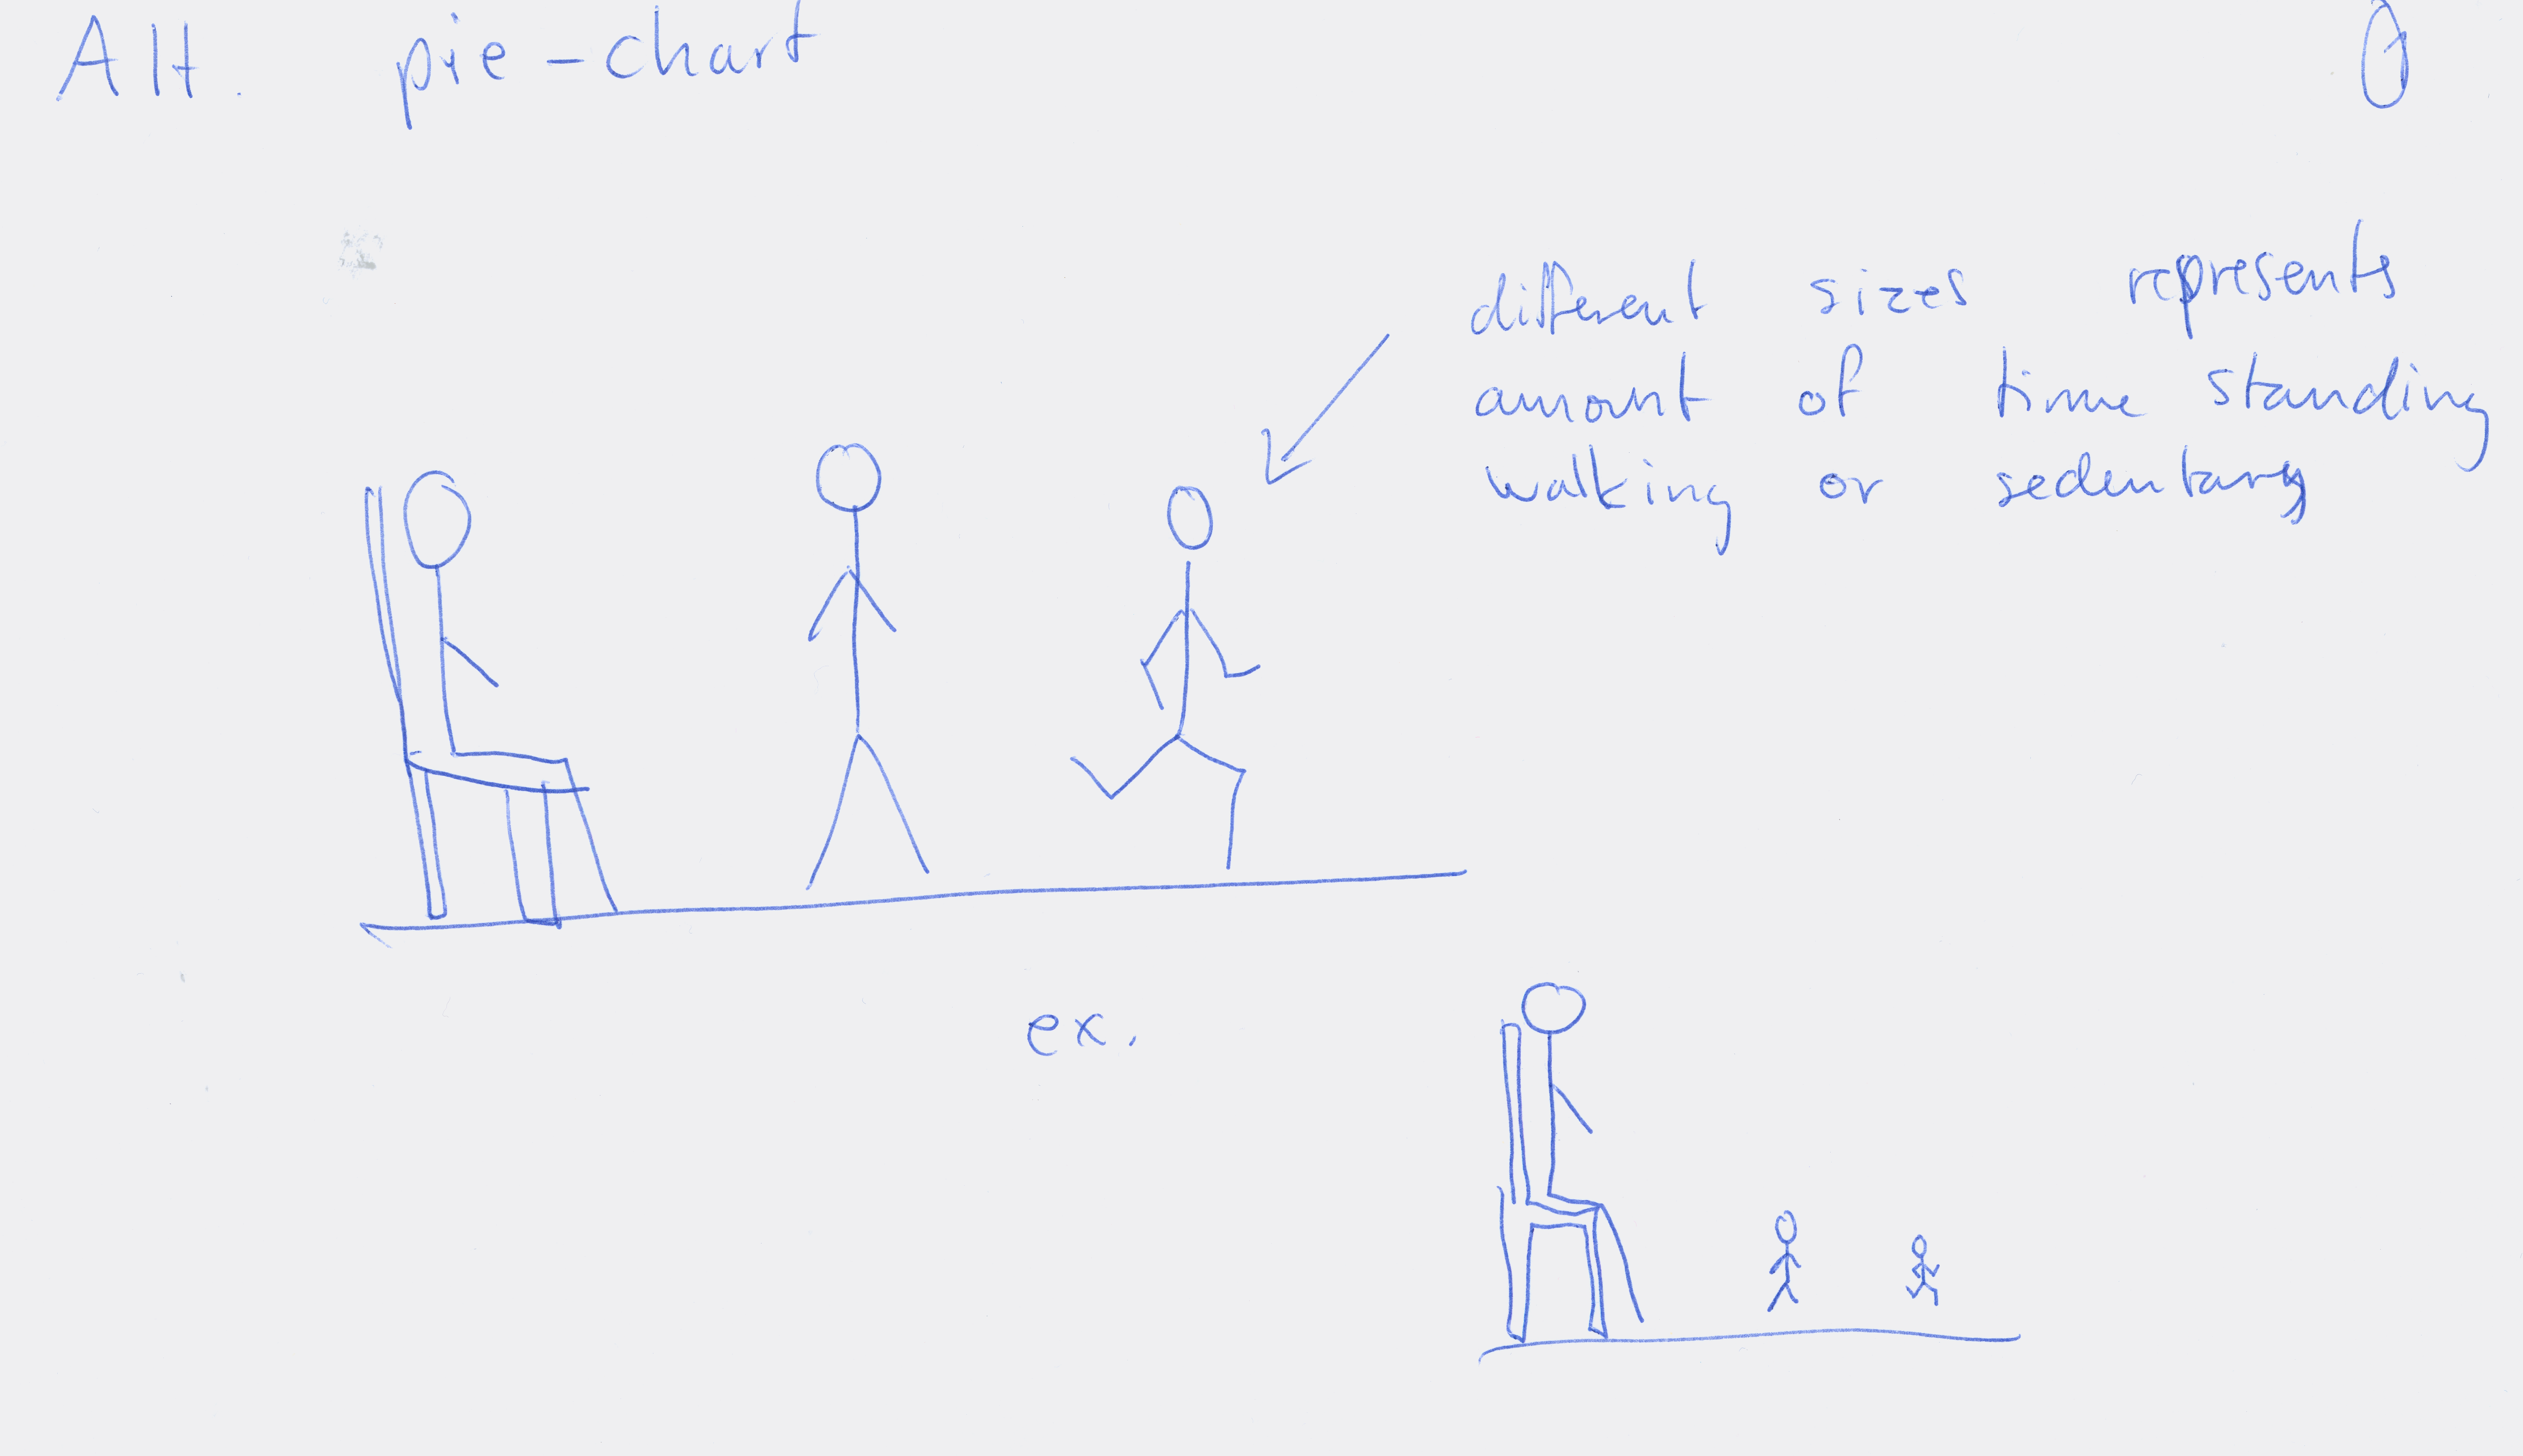
\includegraphics[width=0.7\textwidth]{stickSketch.png}
		\caption{\footnotesize Rough drafts of a symbolic "pie chart"}
		\label{fig:symbolicPie}
\end{figure}

\subsubsection{Ball chart}
Another approach, is to include some more details into a pie chart style, by using balls instead of normal pie slices. Each ball represents an interval of one of the classifications, so that many balls of one colour both represents the amount of that behaviour and shows how long each period of that behaviour was. Figure %need a figure here
shows an example of such a graph. The benefit with this type of graph is that you easily can identify if you have long stretches of sedentary behaviour. Taking small breaks with active behaviour can help ``split up'' those balls, which may be beneficial for your health. Adding interactivity to the chart you can select each ball and see what time it corresponds to. This way you can quickly find the larger balls and identify what time of the day this behaviour occurred. 
%I don't even know man, fuck you.

\subsection{Timeline}
Timeline visualisations are effective at illustrating when various activities occurred during the day. The illustration uses a long horizontal bar that has different colours for different behavioural classification. Such a bar can be used to identify points during the day where the subject is in a sedentary position for too long. By looking at multiple days, the user can detect patterns in the day where he needs to be more active.

\subsubsection{Continuous}
One approach to this visualization is to create a continuous timeline that contains every little detail of behaviour, see figure \ref{fig:timelineContinuous}. The continuous timeline is useful for quickly identifying periods of the day with unsatisfactory behaviour, but the detail can also be distracting and make it harder to read the graph. Adding a fourth colour to highlight long periods of sedentary behaviour can make the timeline easier to interpret.

%Perhaps represent the block based one instead?
\begin{figure}[h!]
	\centering
		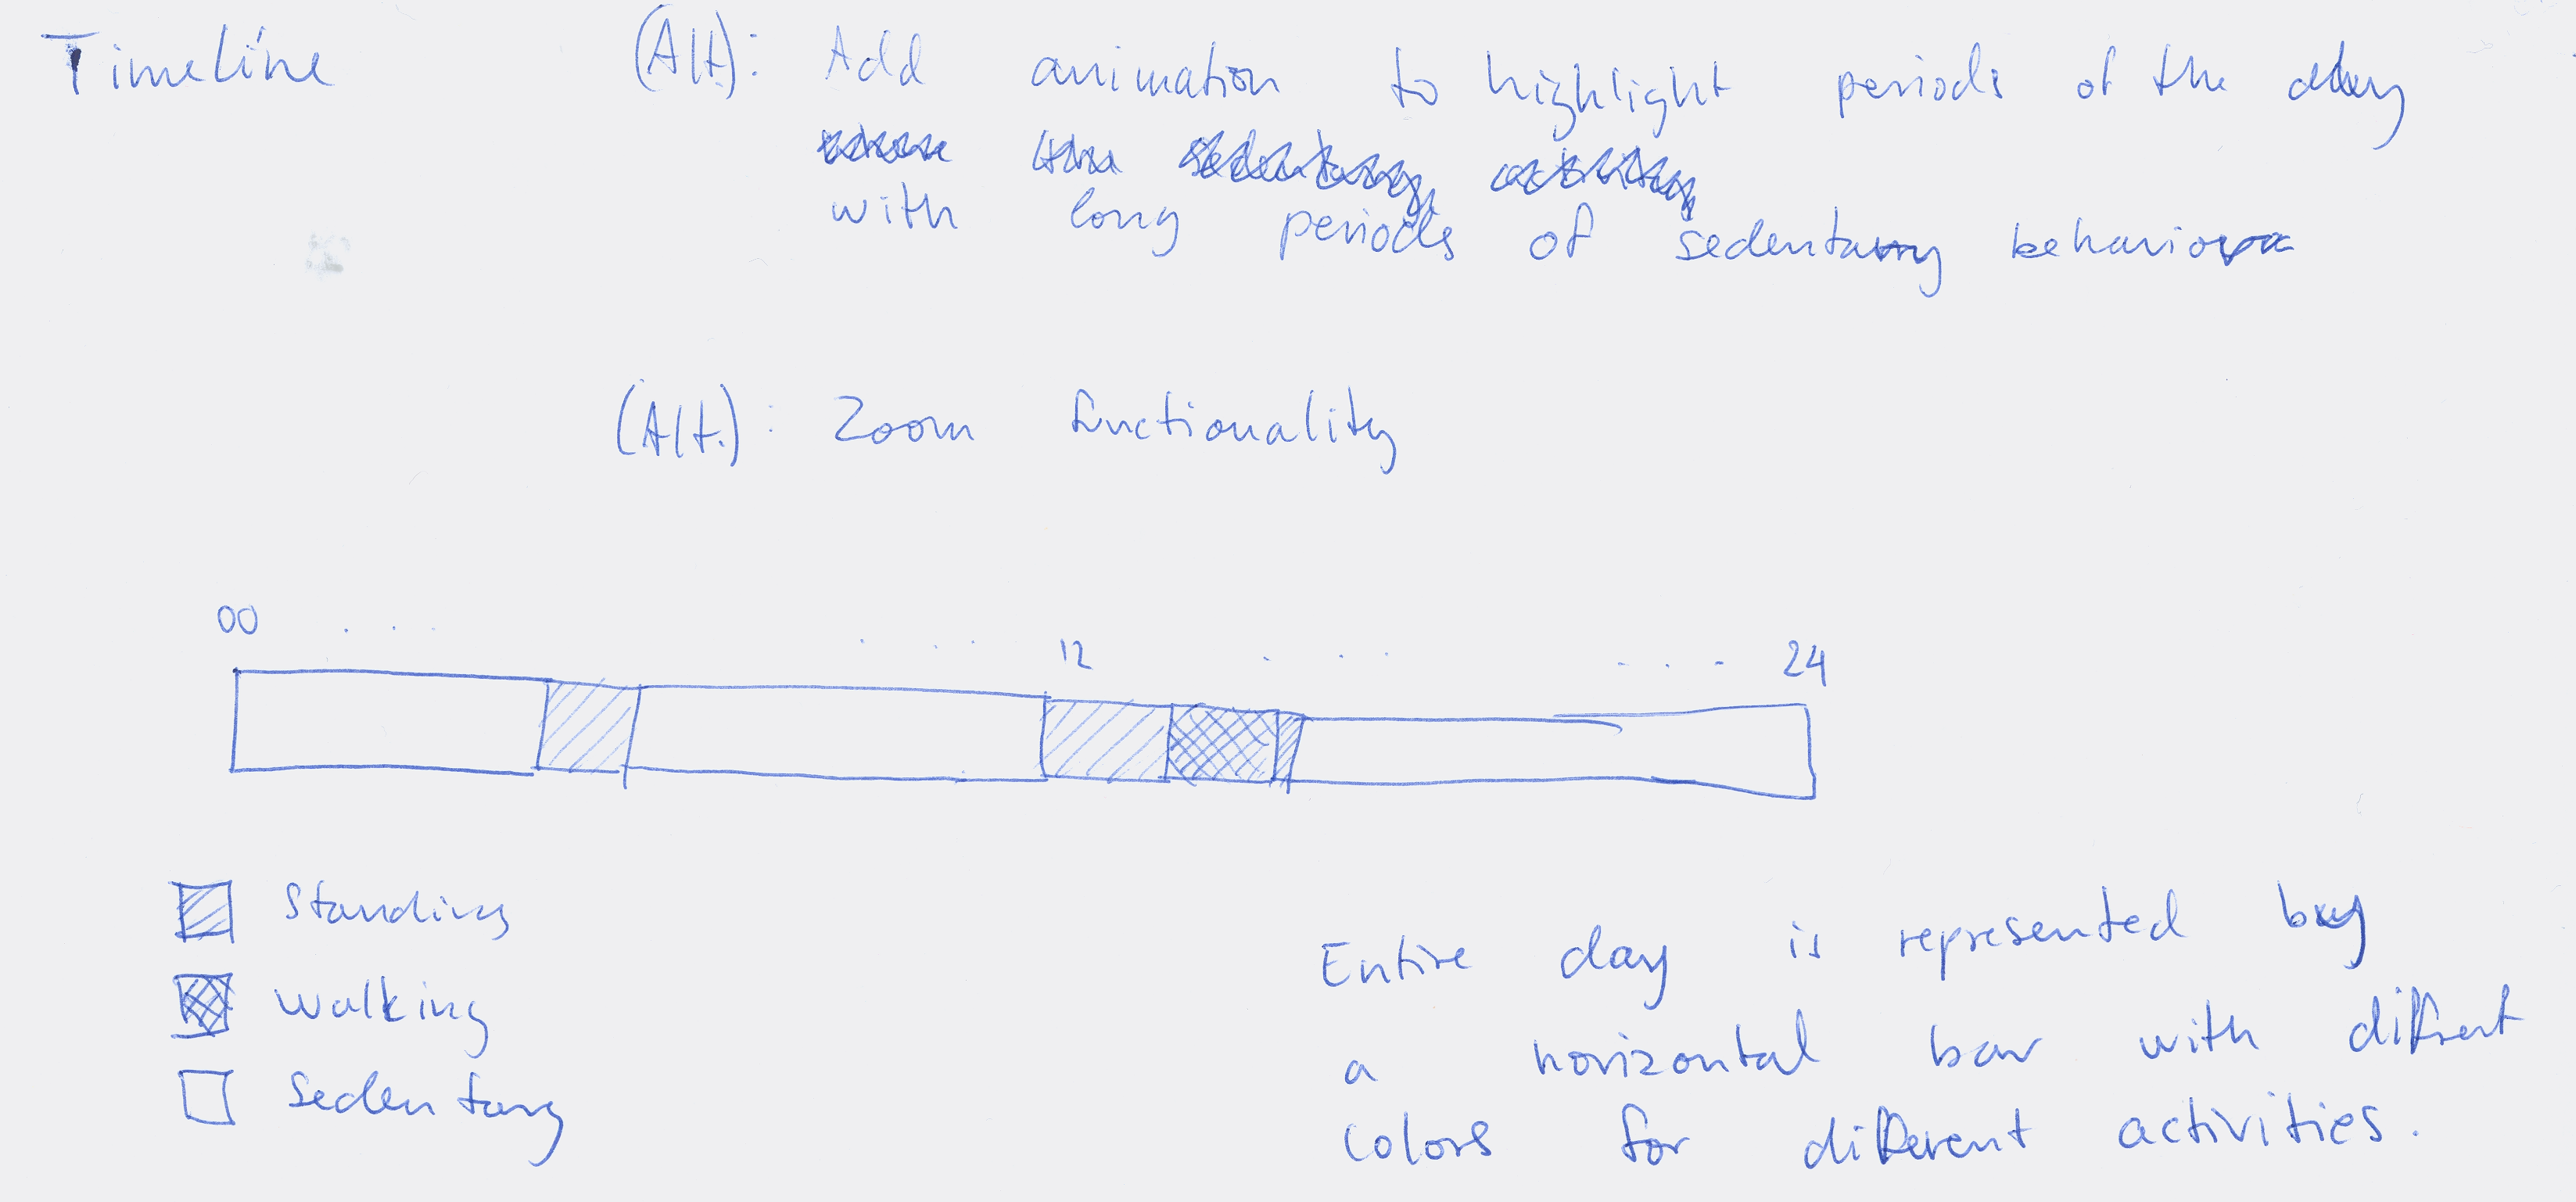
\includegraphics[width=0.7\textwidth]{continousTimelineSketch.png}
		\caption{\footnotesize Timeline with hour blocks}
		\label{fig:timelineContinuous}
\end{figure}
%Does this part need more of an introduction?
%Why would you make it less formal?
%Skrevet det litt om for å gjøre det mindre formelt
We came up with a suggestions to represent the passing of time during a day by using an animated timeline and stick figures. The timeline will be drawn in real time while stick figures simultaneously perform the corresponding activities. By displaying the day gradually we hope that the subject will gain a firm understanding of their day. This means that this visualization can not be used to gain a quick overview, but is intended to be used when viewing a day for the first time.

The more motivational approach would be to replace the stick figure with an analogy or metaphor. Instead of a stick figure, a flower could be used. Activity would allow the plant to get sunlight, making it grow. Sedentary positions would make the weather cloudy and the flower would be unaffected.

\subsubsection{Blocks}
Instead of having a continuous scale, a blocked approach can be used, as seen in figure \ref{fig:timelineBlocks}. The timeline would be divided into 24 blocks, each block corresponding to an hour. A gradient colour scale would be used to represent the amount of activity inside the hour block. This should make it easy to identify hours in the day where prolonged sedentary positions are present. Giving feedback about specific hours might make it easier to interpret and make use of the chart, because you are alerted to certain hours of the day where you should be more active.

%Perhaps represent the block based one instead?
\begin{figure}[h!]
	\centering
		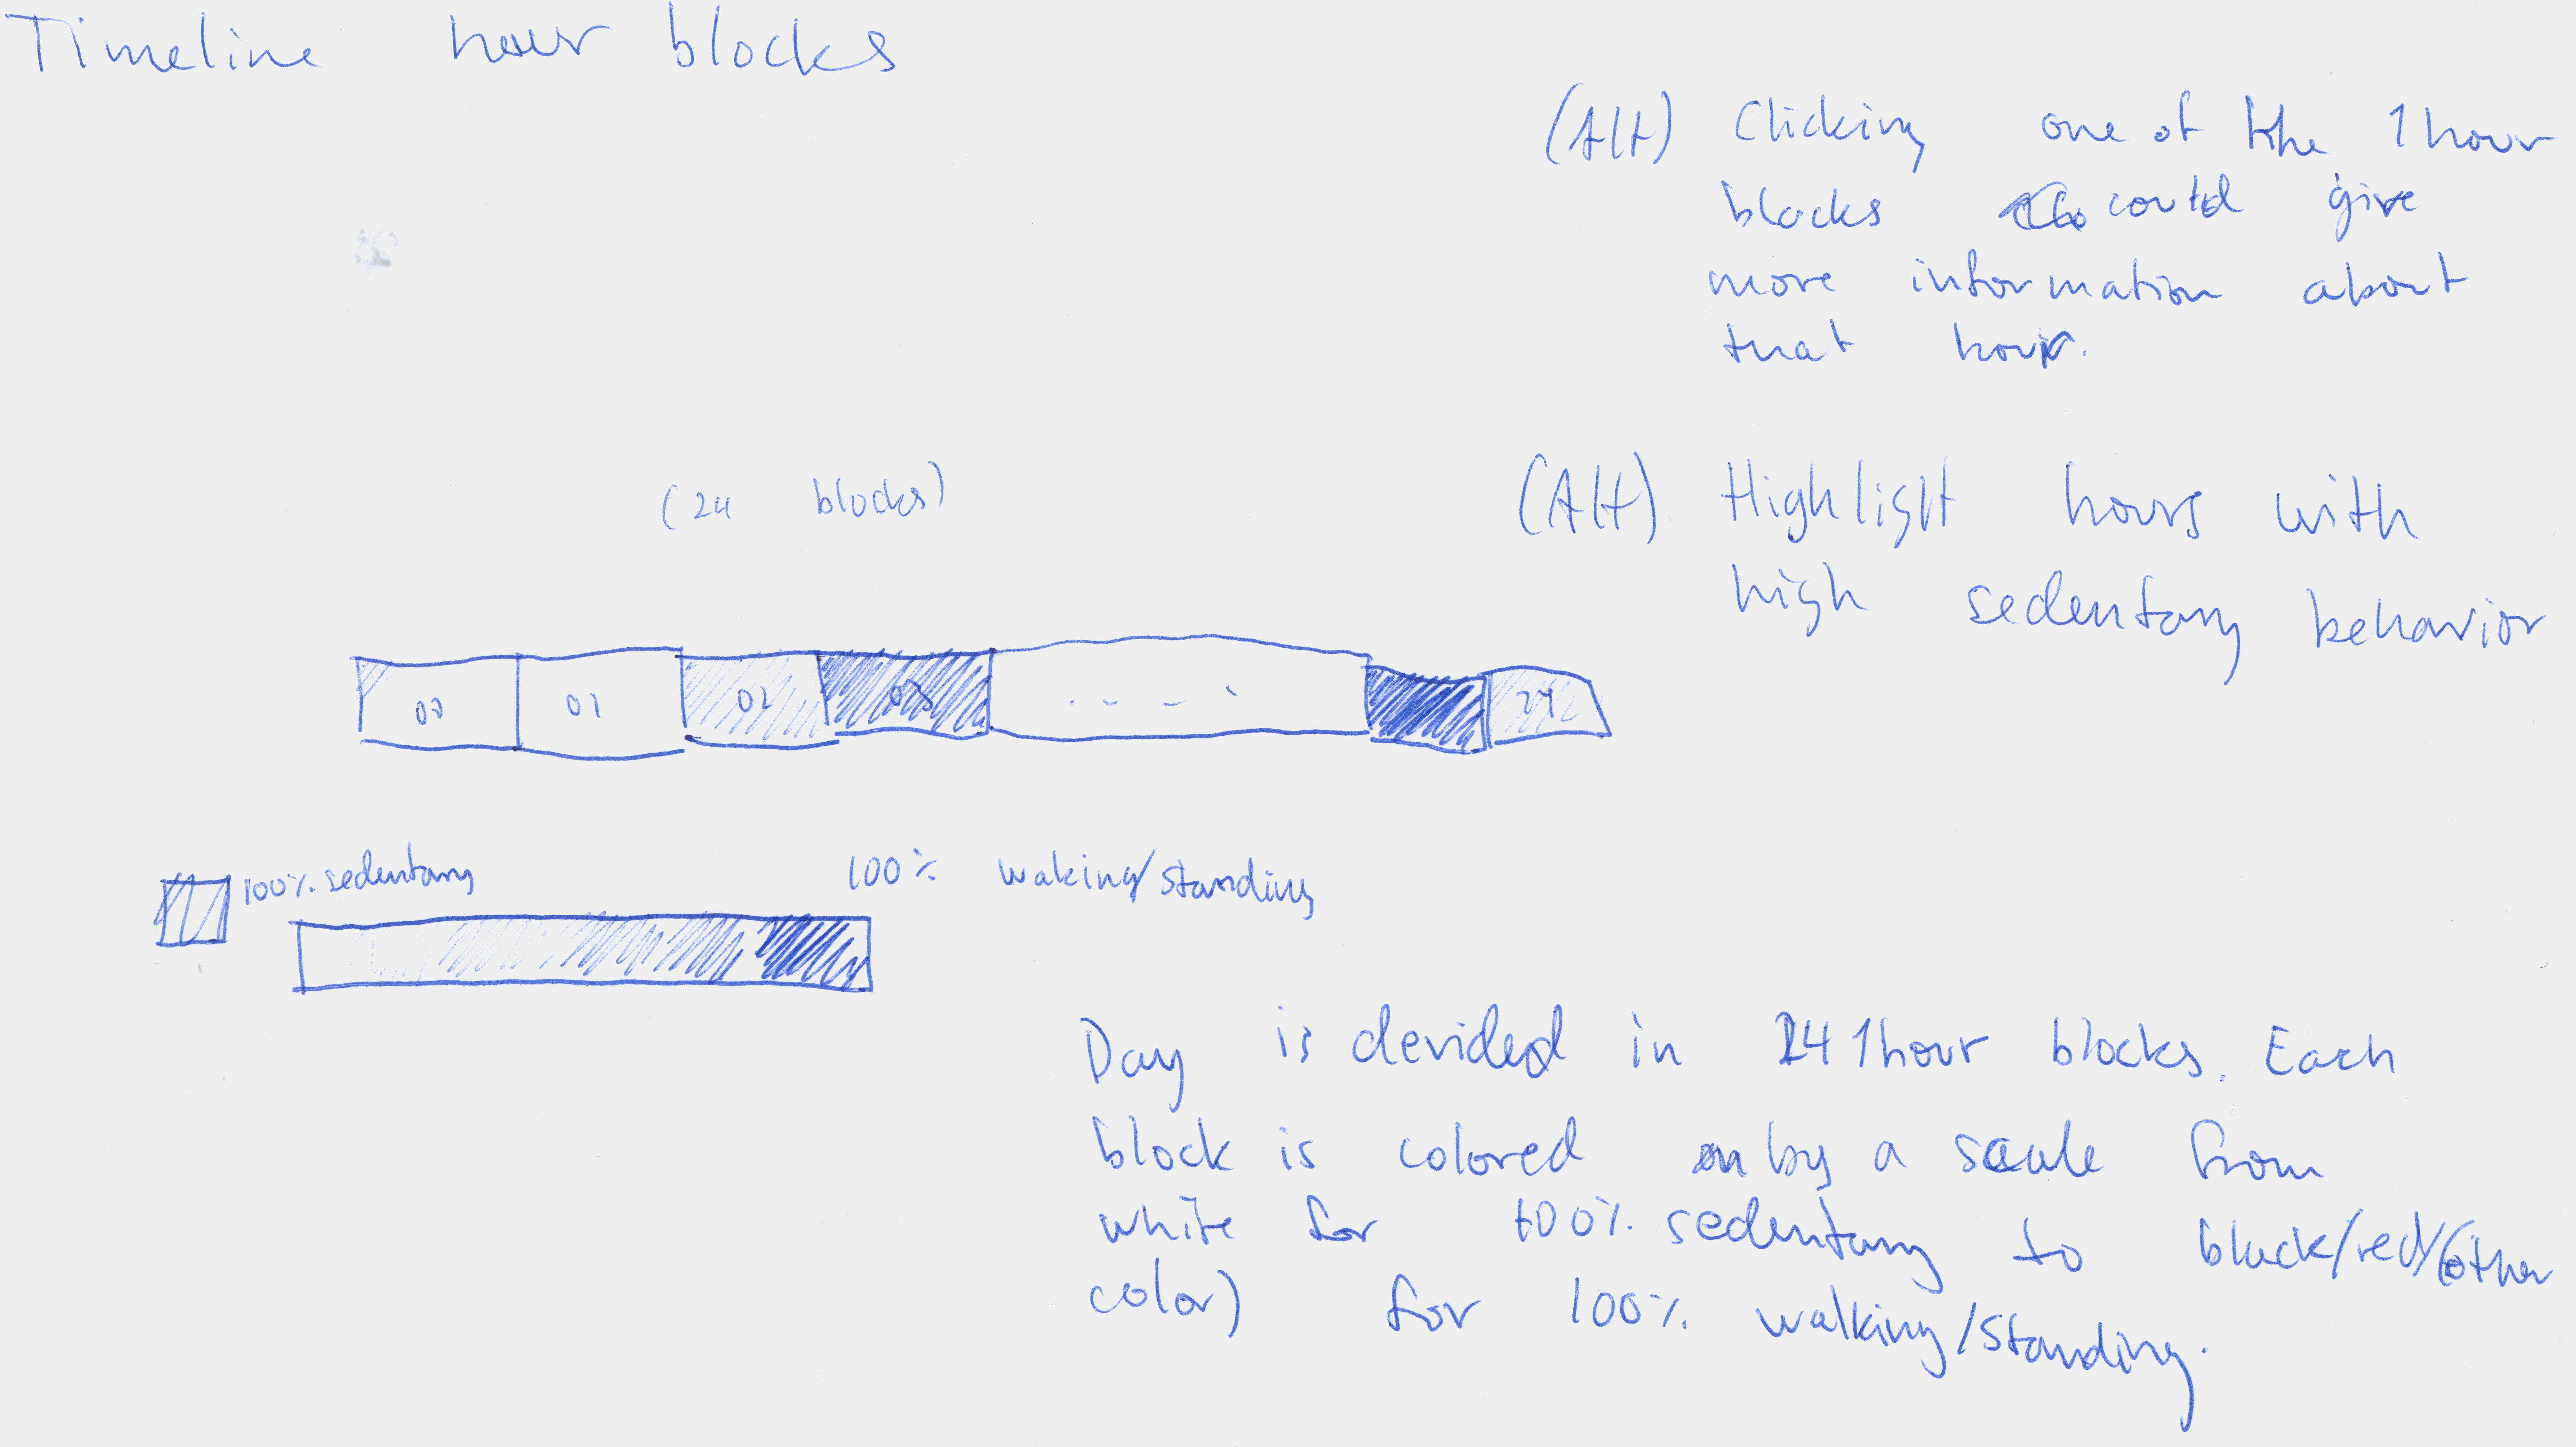
\includegraphics[width=0.7\textwidth]{timelineBlocksSketch.png}
		\caption{\footnotesize Timeline with hour blocks}
		\label{fig:timelineBlocks}
\end{figure}

\subsubsection{Clock}
%Is this part too short now?
A timeline may need some explanation before the user understands it properly. By creating two clocks instead of a long horizontal bar the user can more intuitively understand what the visualization is presenting. Since a clock has only 12 hours, two clocks would need to be drawn. To make it easier to identify day and night, a descriptive background will be added, see figure \ref{fig:clock12}.

\begin{figure}[h!]
	\centering
		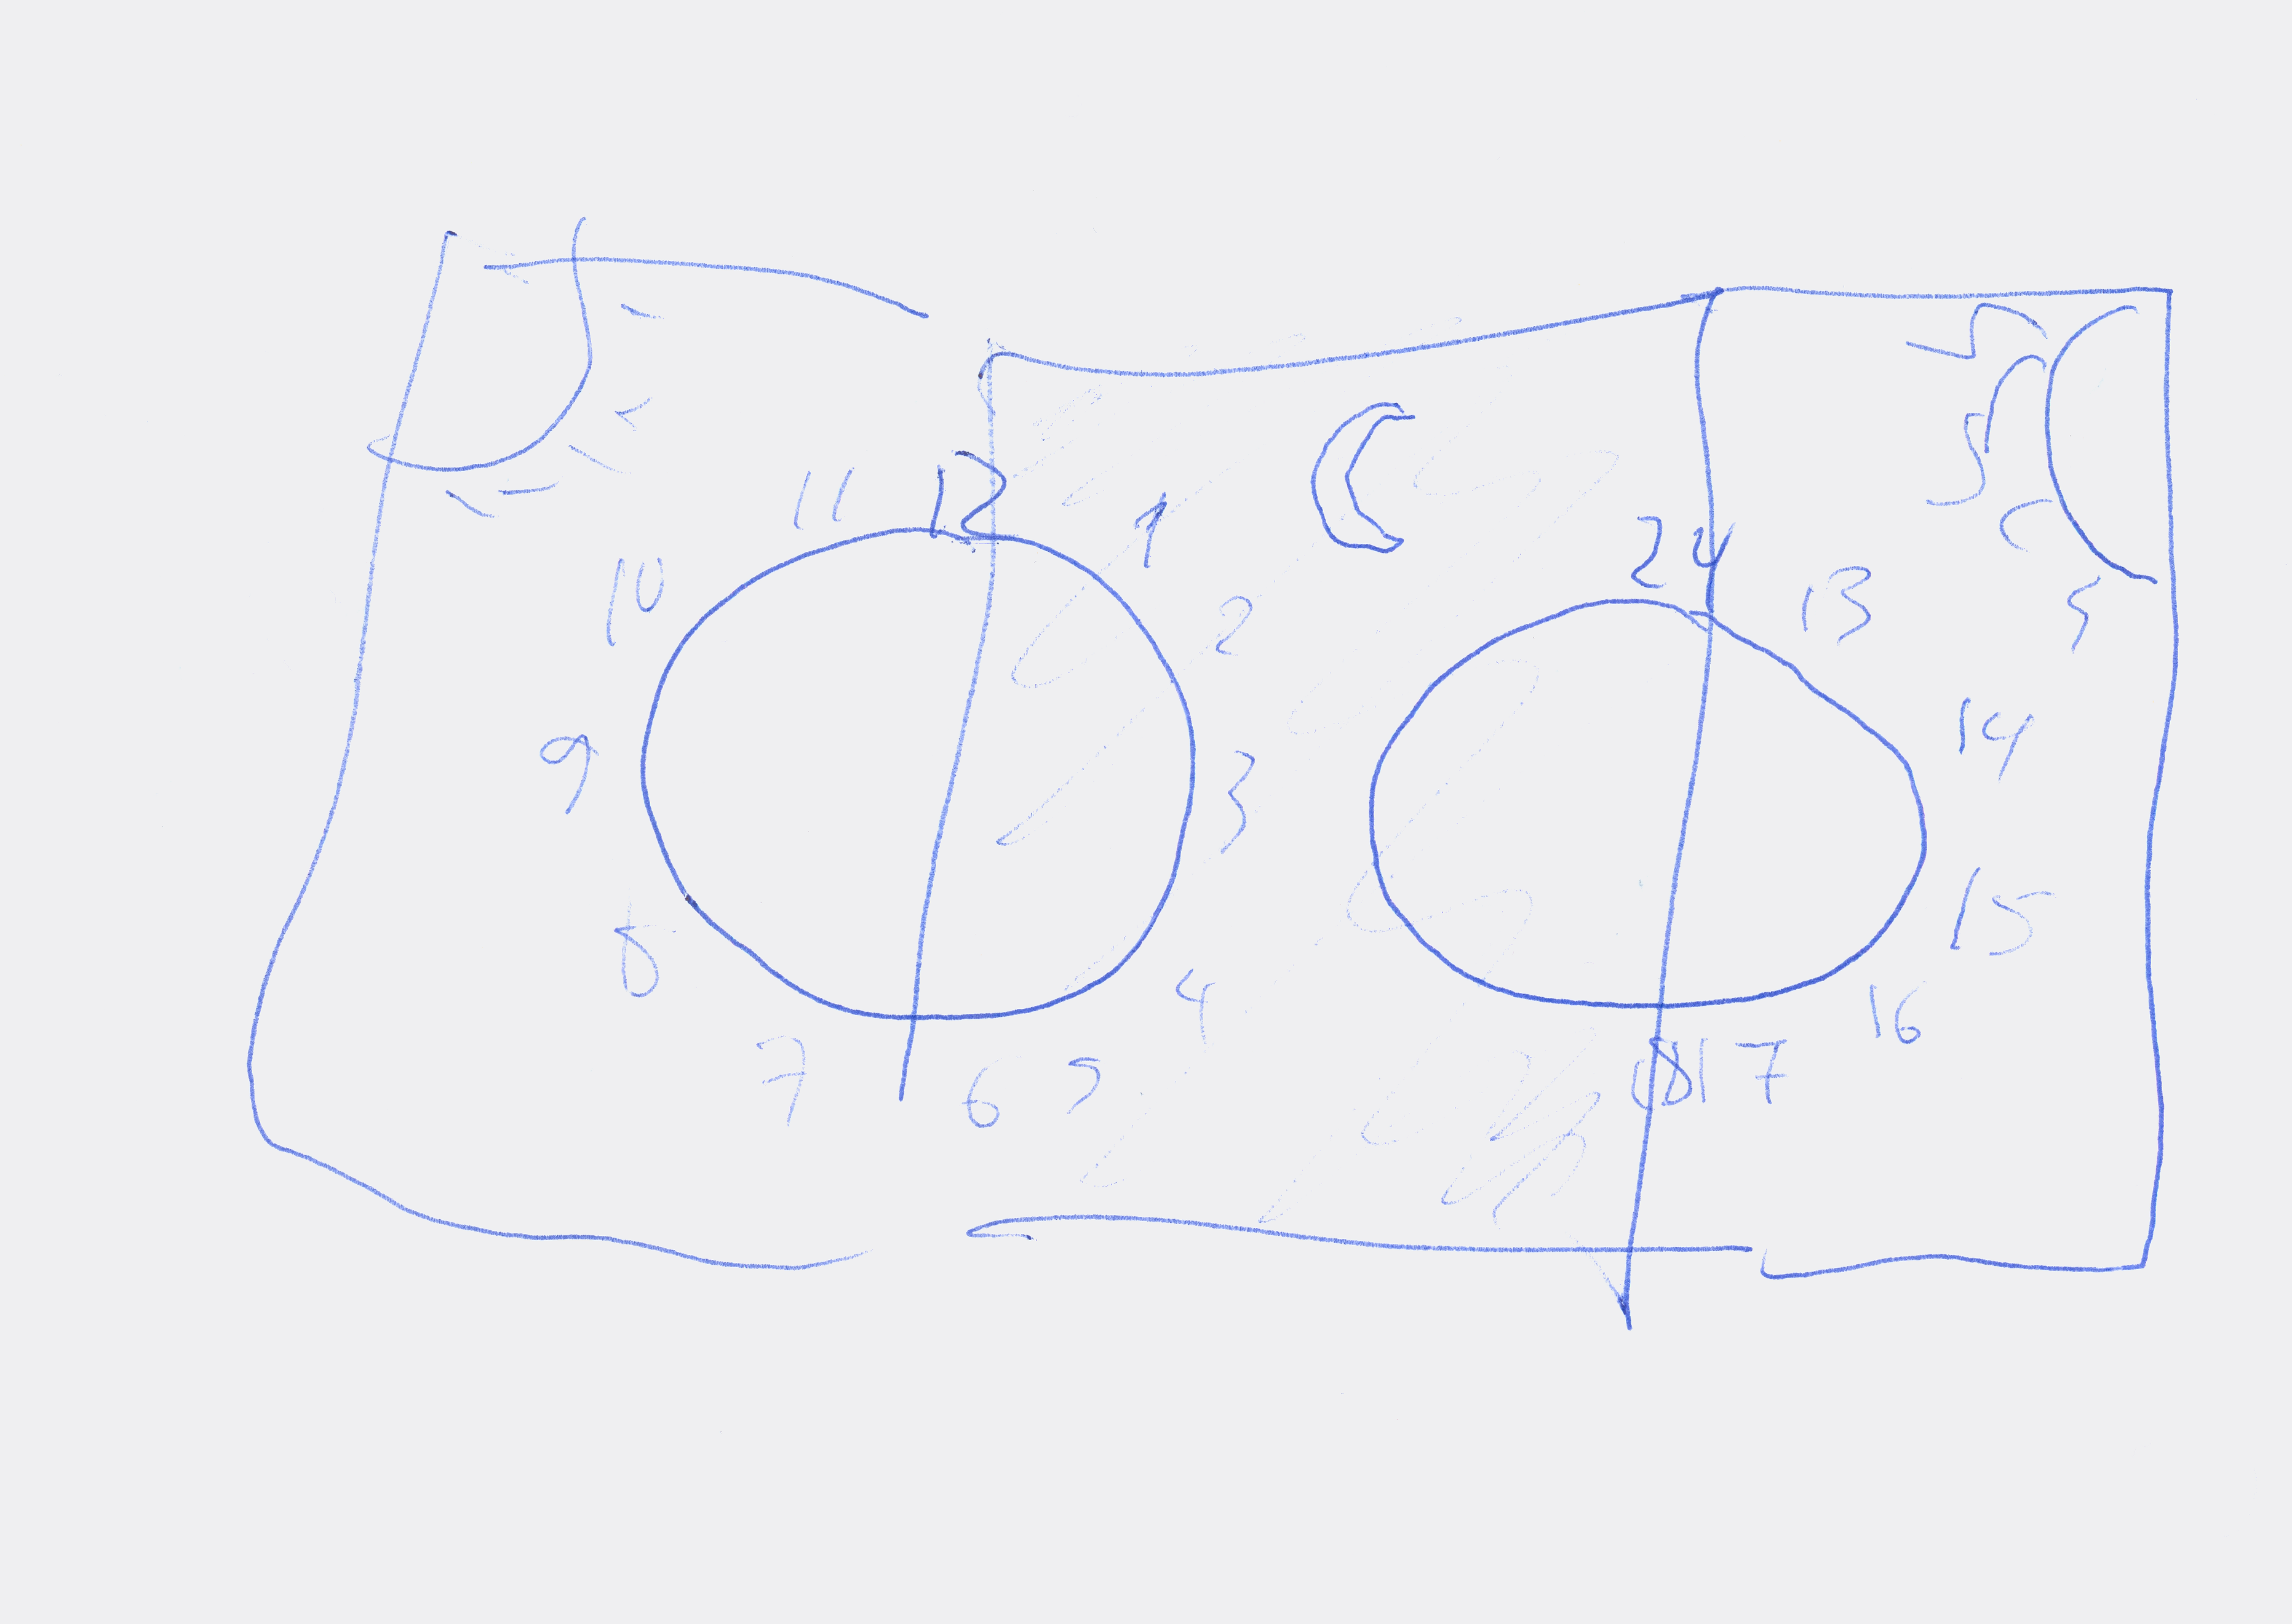
\includegraphics[width=0.7\textwidth]{clock12Sketch.png}
		\caption{\footnotesize Two 12 hour clocks show the activity of the day.}
		\label{fig:clock12}
\end{figure}

Another approach is to use one 24 hour clock, see figure \ref{fig:clock24}. This makes it easier to see the transition between AM and PM, but the users will not be used to seeing a 24 hour clock. This clock will also utilize different background to differentiate between day and night more easily.

\begin{figure}[h!]
	\centering
		
\includegraphics[width=0.5\textwidth]{placeholder.jpg}
		\caption{\footnotesize A single 24 hour clocks show the activity of the day.}
		\label{fig:clock24}
\end{figure}

%Might add a paragraph about highlighting long periods of sedentary behaviour.

\subsection{Week overview}
Getting an overview of the week as a whole can be useful as an introduction. By looking at an overview the user can quickly identify problem days that can then be investigated further. These charts could also be used as the top level of an interactive application. Each day could then be clicked to show either a timeline or pie chart. 

\subsubsection{Day classification}
By calculating the overall activity level and classifying the days into three categories the user can easily see which days he need to be more active and which days the activity level is satisfactory. In our sketch, see figure \ref{fig:smileyWeek} the three different classifications are illustrated by smilies (smiling face for active days, and sad face for inactive days).

\begin{figure}[h!]
	\centering
		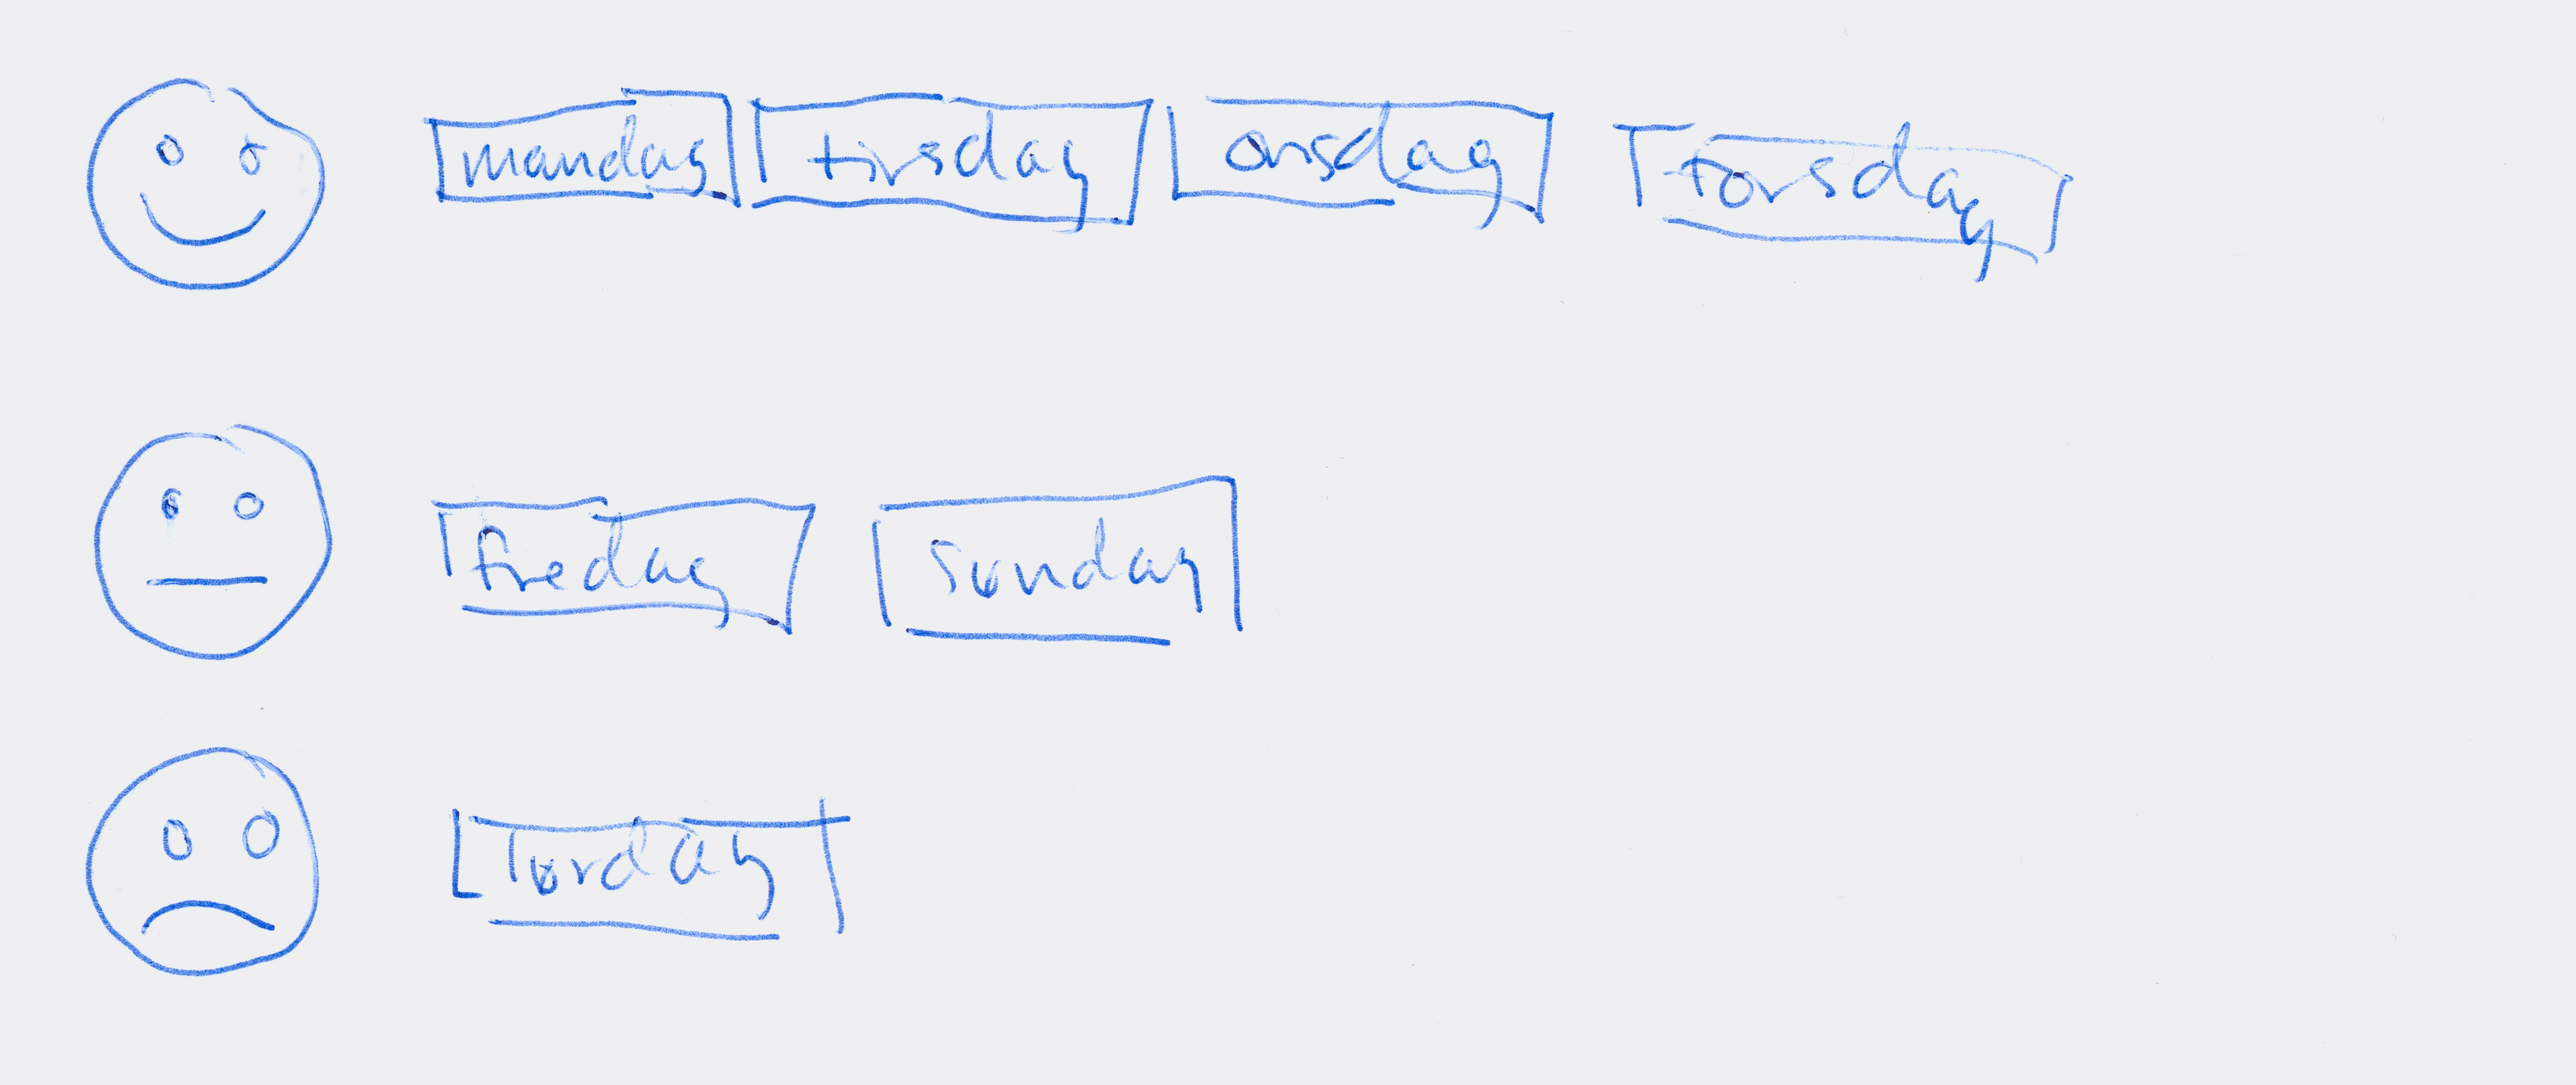
\includegraphics[width=0.7\textwidth]{smileyWeekSketch.png}
		\caption{\footnotesize Week overview with each day classified into one of three categories.}
		\label{fig:smileyWeek}
\end{figure}

A more complex version of the above chart, see figure \ref{fig:detailedWeek} is to show a square for each day, while still using the same classification into sad and happy smilies. Each day square will then contain 24 smaller squares that represent each hour of the day. The small hour square are coloured with a gradient to show the activity level that hour.

\begin{figure}[h!]
	\centering
		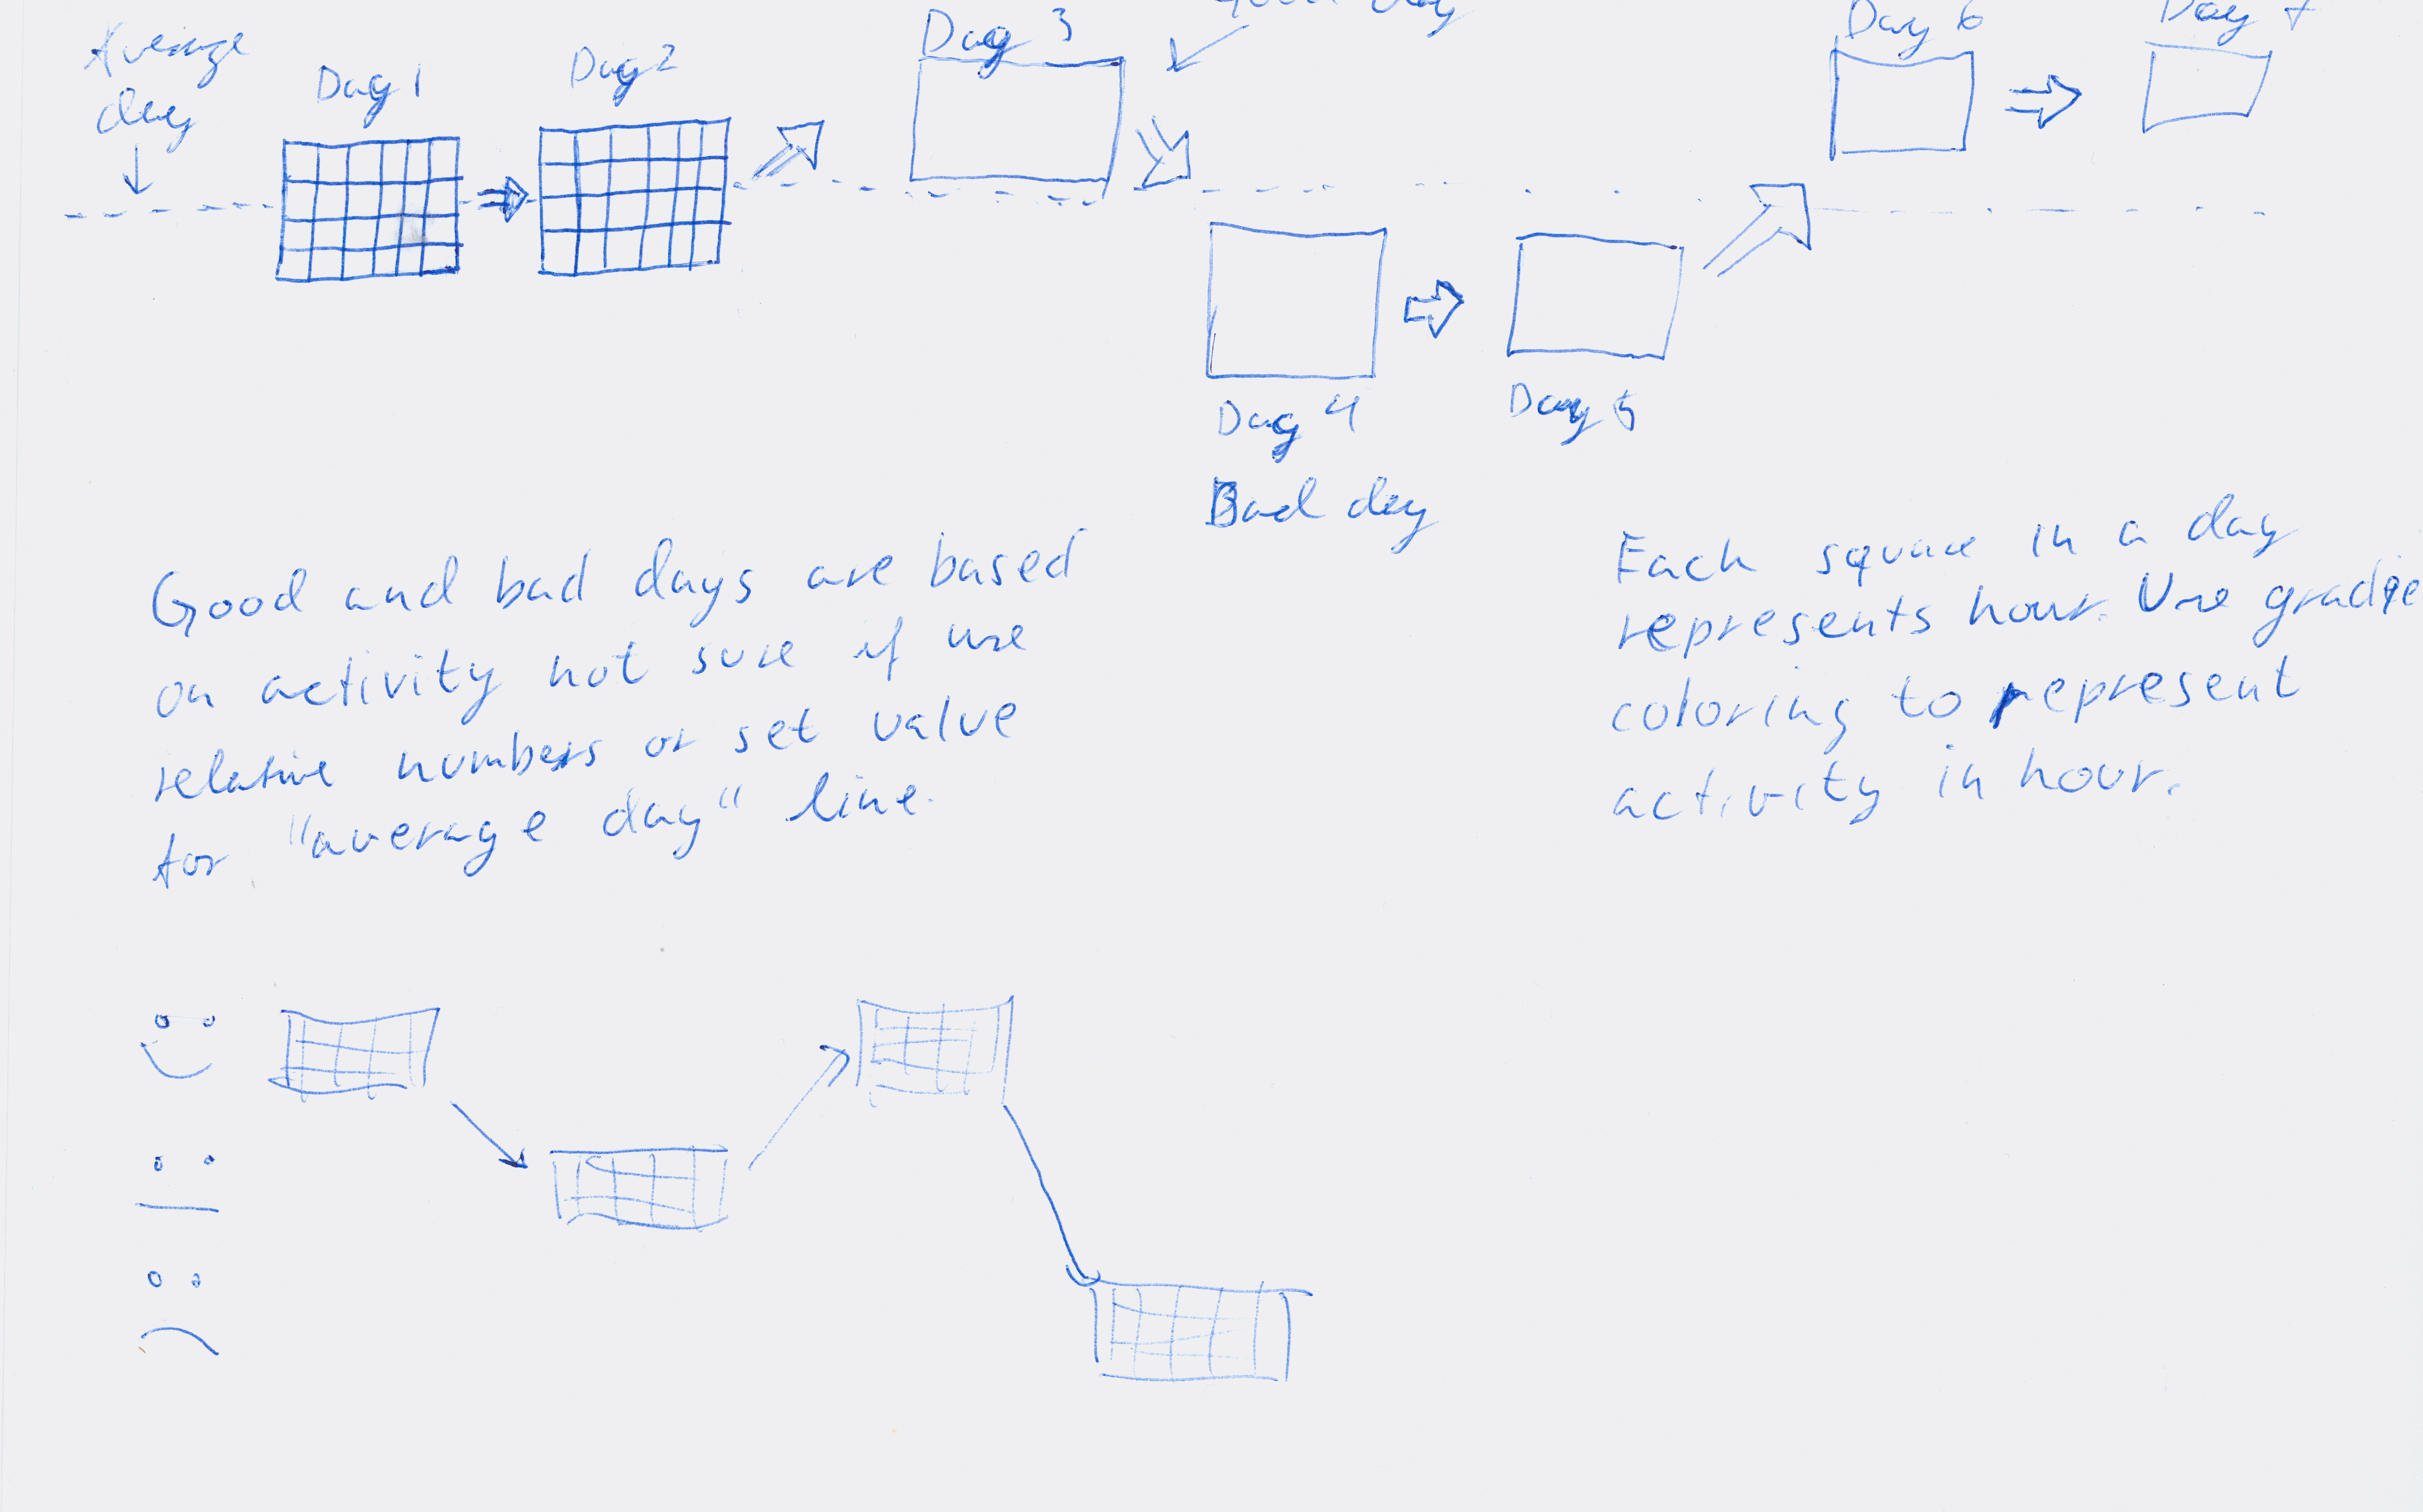
\includegraphics[width=0.6\textwidth]{detailedWeekSketch.png}
		\caption{\footnotesize Some explanation here.}
		\label{fig:detailedWeek}
\end{figure}

With this chart you can get an overview of the week as a whole, and identify what hours of the inactive days had the most sedentary behaviour. 

%This should be moved I guess, or the section should be renamed away from prototype to something like "Graphs" I am not sure.
\section{Hypothesis}
During the initial creation of the graphs %(rename to workshop?) 
we discussed what purpose each graph was designed to serve. A set of hypothesis were created to facilitate our assumptions and allow them to be confirmed or disproved. The graphs are primarily compared to those within the same category as they have been divided to in section \ref{sec:initialGraphs}

\begin{description}
\item[Hypothesis F1:] The stick figures will make the symbolic box chart more intuitive than the pie chart, removing the need for legends.

\item[Hypothesis F2:] The bubble chart is effective at getting the overall distributions of time spent in the different activities.

\item[Hypothesis F3:] The bubble chart makes it easy to identify interval of high sedentary time.

\item[Hypothesis F4:] The pie chart is more likeable then the other fractional charts.

\item[Hypothesis T1:] The blocked timeline makes it easier to identify hours of the day with high sedentary instead of the continuous timeline.

\item[Hypothesis T2:] The extra detail in the continous timeline is useful when going through the patients day.

\item[Hypothesis T3:] Two 12 hour clocks are easier to interpret then a single 24 hour clock.

\item[Hypothesis T4:] It is easier to analyze the day using a timeline than a clock layout.

\item[Hypothesis T5:] The highlighting makes identify periods of high sedentary behaviour easier.

\item[Hypothesis T6:] The switch view function is useful for comparing days quickly

\item[Hypothesis W1:] The week is useful for quickly identifying days with high sedentary behaviour.

\item[Hypothesis W2:] The extra information in detailed week is not necessary in a overview setting.

\end{description}



\section{Findings}

\subsection{Purpose}
KOMMENTAR: BLIR VELL FEIL Å KALLE DETTE EN SCENARIO, er PURPOSE ET BEDRE ORD!?

Initially we had given the premise of only one scenario to the participants: "The visualizations are to be used during a consultation with a patient who has worn a mobility-sensor for a week."During the focus group it became apparent that the participants saw additional ways our visualizations could be used.

\subsubsection*{S1 - Partners}
Patients are not the only ones that would benefit from appropriate visualisations for the sensor data. Several times the participants mentioned how a certain visualisation would be beneficial to third parties or partners such as rehabilitation departments or home services. The purpose would be to identify days and hours where the patient did not have enough activity. %Visualizations mentioned as fitting for this were F3 (Bubblechart), T1(Blockedtimeline), and T4 (24 hours clock).

\subsubsection*{S2 - Motivation}
Something that seemed to be the prime concern of participants was how to motivate patients and achieve their goals. Avoiding to much emphasis on the bad days was important as the patient could be discouraged, but rather highlighting the good days and identify why these were good. A personalized daily goal played a big part in motivating the patient and keeping them going. %Dean: Tror ikke vi hadde noen visulisasjoner som oppfyller dette, hva sier du knut?

\subsubsection*{S3 - Categorizing days}
In one of our visualizations we presented the idea of categorizing days into three categories based on the users activity level. The participants received the idea well and perceived it as a help to quickly identify which days they should focus on, but mentioned that this was not something they would necessarily use with a patient. 

\subsubsection*{S4 - Hours}
The participants were interested in how the activity of a patient is distributed through the day. This way they could identify hours of the day where the patient was active, allowing them easily to analyse if there is room for improvement. Two of the participants mentioned that they were also interested to see if the patient was active when he should be sleeping, and if this could be a cause to their low activity during the day.

\subsubsection*{Generell oversikt}
TROR IKKE DENNE SEKSJONEN ER RELEVANT FOR OSS, TAR DET MED SOM ET NOTAT SÅ JEG HUSKER PÅ DET.


\subsection{Table}
A table was created to help link the various scenarios to our graphs so we could quickly identify if all of our visualizations covered the aforementioned scenarios.
\begin{center}
\begin{table}[h!]
\begin{tabular}{cc|c|c|c|c|c|c|c|c|c|c}
	\cline{2-10}
	 & \multicolumn{9}{ |c| }{Visualisation} \\ \cline{1-10}
    \multicolumn{1}{ |c| }{Scenario} & U1 & U2 & F1 & F2 & F3 & T1 & T2 & T3 & T4 \\ \hline
     \multicolumn{1}{ |c| }{Motivating Patient} & - & - & - & - & - & - & - & - & -  \\ \hline
     \multicolumn{1}{ |c| }{Identifying days} & + & + & - & - & + & + & - & - & -  \\ \hline
     \multicolumn{1}{ |c| }{Finding hours to improve} & - & - & - & - & - & + & - & - & +  \\ \hline
	 \multicolumn{1}{ |c| }{Showing partners} & - & - & - & - & + & + & - & - & +  \\
    \hline
\end{tabular}
\end{table}
\end{center}
